\section{Full Loss Trajectories and Expanded Experimental Scope}
\label{app:loss-trajectories}
\paragraph{Frozen plotting and selection protocol.}
Every plotted value comes from a retained JSON trajectory. The figure audit records source paths, SHA-256 digests, the selected metric, point counts, and the last observed abscissa. Classification selections use terminal-100 validation accuracy among completed 1000-epoch trials. The scientific panels restrict both methods to rank 64 and choose within that rank using terminal-100 PDE residual; exact-solution errors never select the curve. Seed 42 is used throughout. Archived epoch indices and new one-based epochs are retained separately. Curves are not stretched to a common horizon, and unfinished traces do not enter endpoint or AUC comparisons. No confidence intervals are claimed.
\begin{figure}[!htbp]
\centering
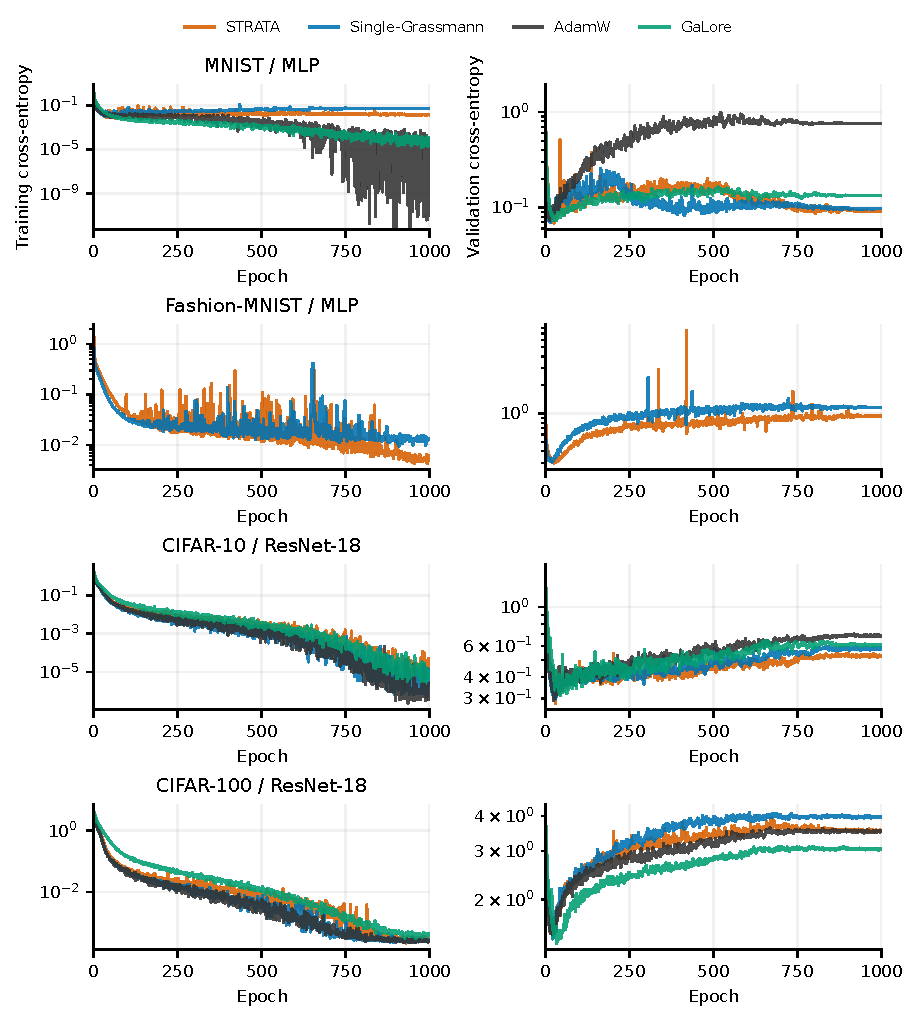
\includegraphics[width=.98\linewidth]{figures/fig_loss_classification_validation.pdf}
\caption{\textbf{Training and validation cross-entropy for the selected classifiers.} Each row is one dataset; left: training loss; right: held-out validation loss. The same selected run supplies both panels. A declining training loss with rising validation loss is retained. Missing Fashion-MNIST baselines are left absent. These are single-seed archived trajectories with unequal baseline search sizes.}
\label{fig:loss-classification-validation}
\end{figure}
\begin{figure}[!htbp]
\centering
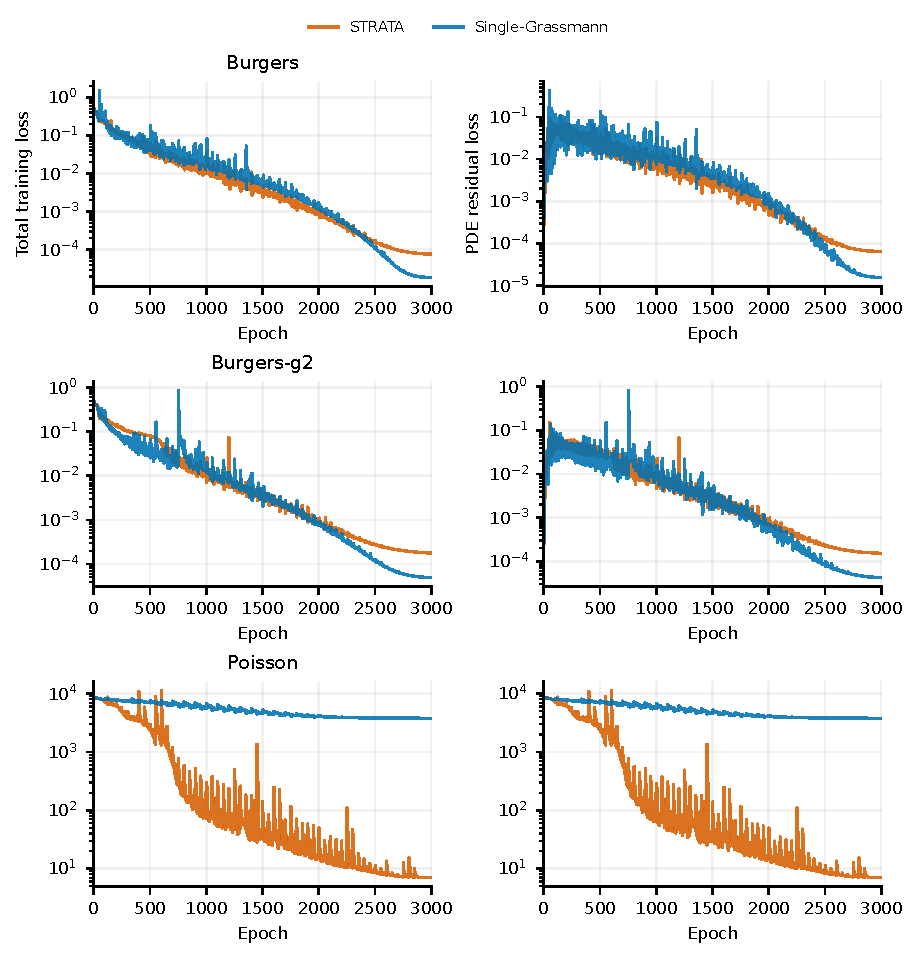
\includegraphics[width=.98\linewidth]{figures/fig_loss_scientific.pdf}
\caption{\textbf{Scientific-ML convergence at a strictly matched maximum rank of 64.} Left: total training loss; right: PDE residual loss. Exact-solution endpoint errors are tabulated separately. Rows: Burgers, Burgers-g2, Poisson. Each method's learning rate is selected by terminal PDE loss within rank 64. For Poisson this gives Single-Grassmann 2.04357 and STRATA 0.18741. The former differs from 2.00280, the rank-32 winner of the pooled-rank Single-Grassmann grid. Neither exact-solution error nor a favorable intermediate point selects a run.}
\label{fig:loss-scientific}
\end{figure}
\begin{figure}[!htbp]
\centering
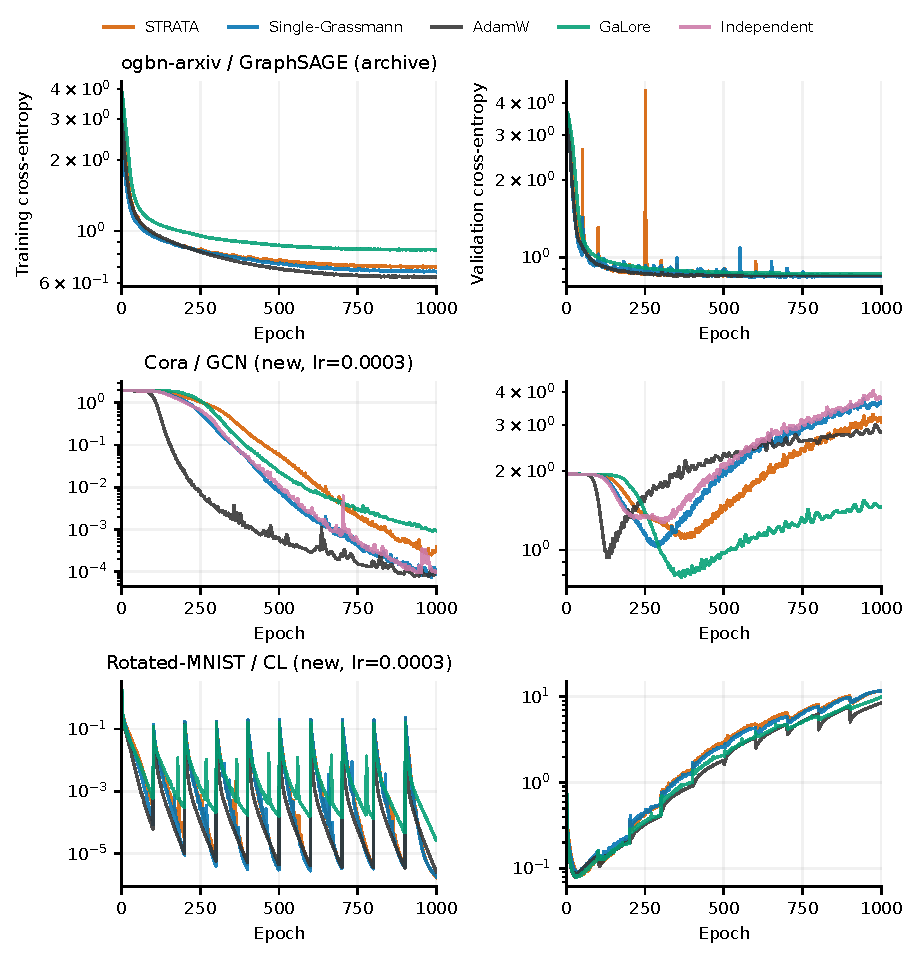
\includegraphics[width=.98\linewidth]{figures/fig_loss_graph_continual.pdf}
\caption{\textbf{Graph and continual-learning loss trajectories.} Left: training cross-entropy; right: validation cross-entropy. Rows show archived ogbn-arxiv, newly completed Cora/GCN configurations at the fixed rate $3\times10^{-4}$, and newly completed Rotated-MNIST fine-tuning configurations at that same fixed rate. In continual learning the held-out loss averages seen tasks, whose set grows at task boundaries; it is not the loss on an unchanging distribution. Only completed configurations are included in these panels.}
\label{fig:loss-graph-cl}
\end{figure}
\begin{figure}[!htbp]
\centering
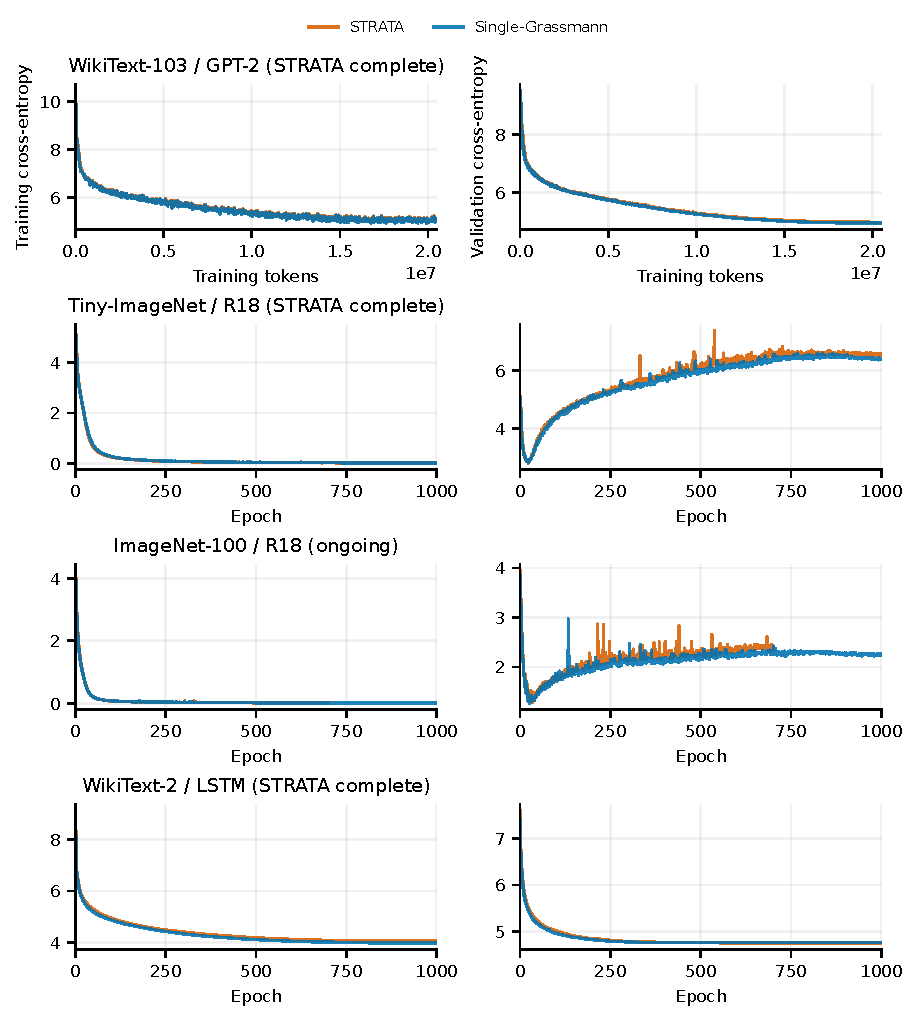
\includegraphics[width=.98\linewidth]{figures/fig_loss_ongoing.pdf}
\caption{\textbf{Large-task trajectories and configuration completion status.} Left: training loss; right: validation loss. Rows show WikiText-103/GPT-2, Tiny-ImageNet/ResNet-18, ImageNet-100/ResNet-18, and WikiText-2/LSTM at rate $3\times10^{-4}$. GPT-2 uses actual training tokens; the other rows use observed epochs. Each WikiText-2 epoch covers the complete next-token training corpus. A title marks any completed STRATA configuration; missing methods and unfinished searches do not become completed comparison cohorts. Other traces stop at their last observed epoch. A missing method has no available trace at the snapshot. The different language tokenizations also prevent interpreting perplexity across the two language-model rows as a matched comparison. These traces do not establish a family-level advantage.}
\label{fig:loss-ongoing}
\end{figure}
\begin{figure}[!htbp]
\centering
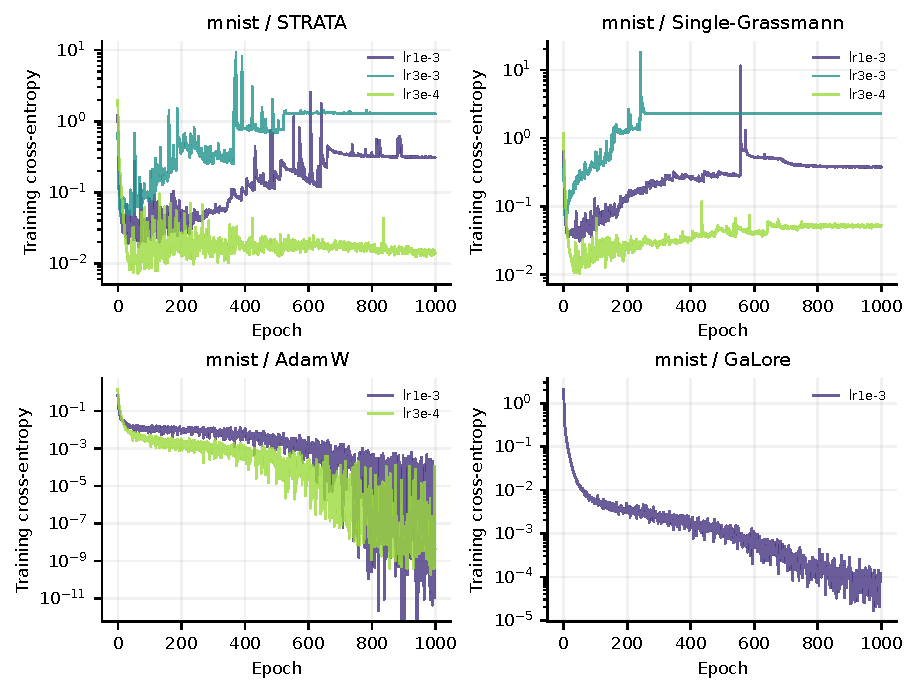
\includegraphics[width=.98\linewidth]{figures/fig_loss_grid_mnist.pdf}
\caption{\textbf{All completed MNIST classifier-grid training losses.} Separate panels show methods; lines show all available completed learning-rate trials. Poor configurations are retained. A 397-epoch partial GaLore trial is excluded from the complete-grid view.}
\end{figure}
\begin{figure}[!htbp]
\centering
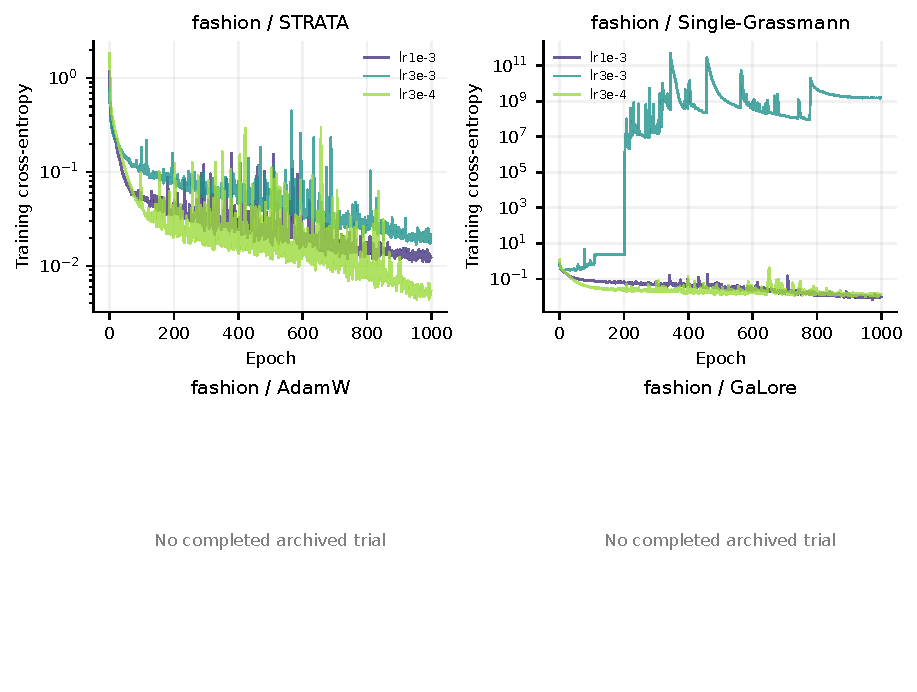
\includegraphics[width=.98\linewidth]{figures/fig_loss_grid_fashion.pdf}
\caption{\textbf{All completed Fashion-MNIST classifier-grid training losses.} Missing archived AdamW/GaLore grids are absent. The unstable Single-Grassmann trial remains visible rather than being removed from the learning-rate matrix.}
\end{figure}
\begin{figure}[!htbp]
\centering
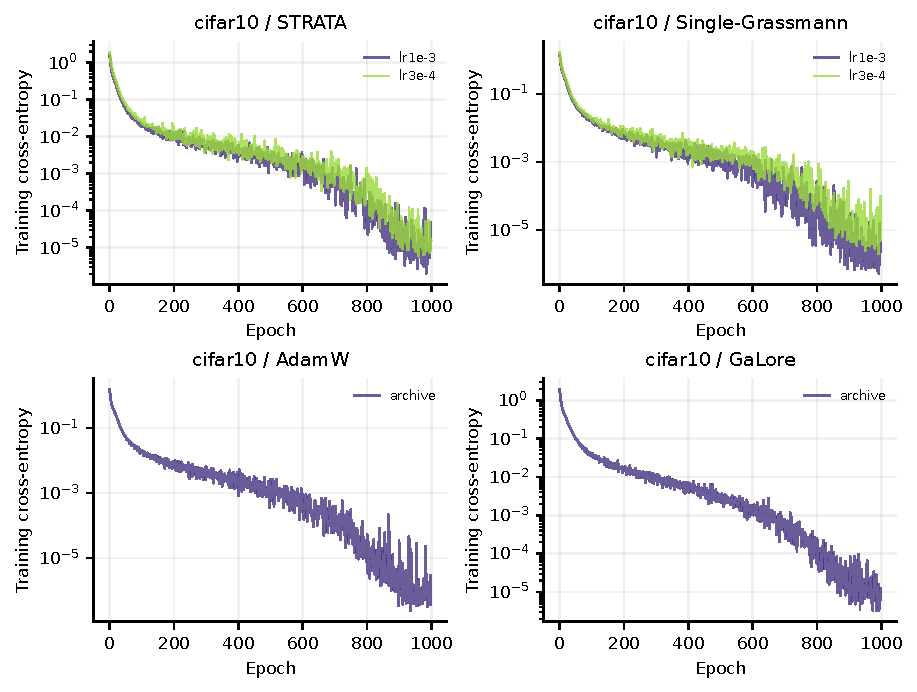
\includegraphics[width=.98\linewidth]{figures/fig_loss_grid_cifar10.pdf}
\caption{\textbf{All completed CIFAR-10 classifier-grid training losses.} STRATA/Single-Grassmann have two available rates; each archived AdamW/GaLore reference has one. These unequal grids are disclosed rather than represented as equal hyperparameter budgets.}
\end{figure}
\begin{figure}[!htbp]
\centering
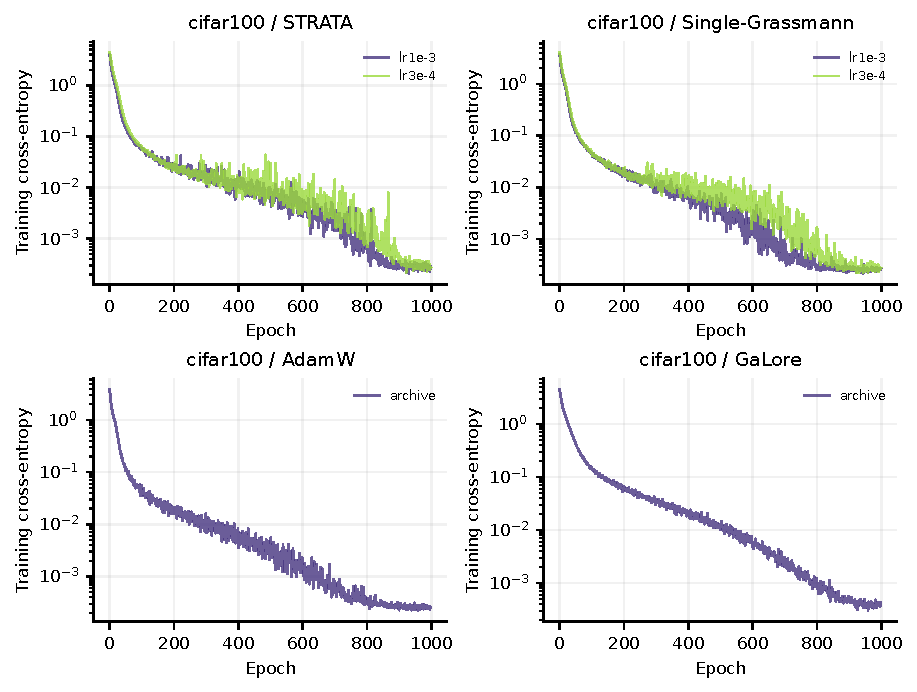
\includegraphics[width=.98\linewidth]{figures/fig_loss_grid_cifar100.pdf}
\caption{\textbf{All completed CIFAR-100 classifier-grid training losses.} The full training paths support optimization diagnostics while the held-out panels prevent interpreting a small terminal training loss as evidence of superior generalization.}
\end{figure}
\begin{longtable}{llrrrr}
\caption{Selected classifier convergence diagnostics. AUC integrates raw training loss over the observed archived epoch indices (0--999); $g_{\rm log}$ is the mean logged gradient norm, not a claim to the exact full-objective gradient. Missing gradient norms were not recorded in those archives and are left absent. Configurations use the selection rule of Figure~\ref{fig:loss-classification}.}\\
\toprule Dataset & Method & Loss AUC & Train loss & Val loss & $g_{\rm log}$\\\midrule\endfirsthead
\toprule Dataset & Method & Loss AUC & Train loss & Val loss & $g_{\rm log}$\\\midrule\endhead
\rowcolor{oursbg}
mnist & strata & 21.9 & 0.0144 & 0.0917 & 4.92 \\
mnist & single & 40.8 & 0.0513 & 0.0969 & 15.8 \\
mnist & adamw & 6.13 & 7.5e-05 & 0.759 & -- \\
mnist & galore & 7.21 & 7.76e-05 & 0.133 & 0.0133 \\
\rowcolor{oursbg}
fashion & strata & 35.2 & 0.0059 & 0.939 & 0.639 \\
fashion & single & 32.4 & 0.0131 & 1.16 & 1.99 \\
\rowcolor{oursbg}
cifar10 & strata & 19.4 & 1.77e-05 & 0.527 & 0.00133 \\
cifar10 & single & 16 & 4.69e-06 & 0.578 & 0.000361 \\
cifar10 & adamw & 17.4 & 3.19e-06 & 0.688 & -- \\
cifar10 & galore & 27.3 & 1.81e-05 & 0.607 & -- \\
\rowcolor{oursbg}
cifar100 & strata & 59 & 0.000286 & 3.56 & 0.00343 \\
cifar100 & single & 49.2 & 0.000261 & 3.98 & 0.00111 \\
cifar100 & adamw & 48.7 & 0.000259 & 3.53 & -- \\
cifar100 & galore & 101 & 0.000407 & 3.05 & -- \\
\bottomrule\end{longtable}


\paragraph{Breadth relative to the ManifoldFlow evaluation.}
The graph additions use custom 256-wide models: attention is single-head, SAGE-style aggregation uses the stated symmetric adjacency, and GCNII-style initial/identity mixing is fixed. These are controlled architecture variants, not reproductions of canonical published endpoints. The reference evaluation combines recurrent language models, tabular and image MLPs, a small Transformer, convolutional heads, component ablations, and scaling diagnostics. Our expanded matrix adds UCI Adult~\citep{uciAdult1996}, Covertype~\citep{uciCovertype1998}, red/white Wine Quality~\citep{uciWine2009} with 256- and 512-wide two-hidden-layer MLPs, and WikiText-2~\citep{merity2016pointer} with two-layer LSTM, two-layer GRU and a two-block Transformer. All five adaptive/projection methods receive rates $3\times10^{-4}$ and $10^{-3}$. Every formal tabular and sequence trial is prescribed 1000 complete epochs. These 110 additional configurations enlarge planned coverage; only completed entries in Appendix~\ref{app:new-completions} count as results.
\paragraph{Preprocessing and language budgets.}
Adult retains the official test split and hashes 10\% of official training for validation. Wine uses separate red/white tasks with target quality $\ge6$; identical full rows share a fixed 70/15/15 hash split. Covertype uses all 581012 records with the same hash split rule. All feature means, scales, and categorical dictionaries are fitted on training only. The WikiText-2 vocabulary is fitted on its official training split, with minimum frequency two and at most 30000 words. Its frozen splits contain 2088628/217646/245569 tokens. Every new sequence epoch visits the complete next-token training corpus; recurrent state is reset between contiguous blocks. This differs explicitly from the separate GPT-2 fixed-ten-step evaluation units. All preprocessing hashes and source revisions are retained.
\paragraph{Mechanistic ablations.}
A further 40 trials compare ten STRATA variants on Adult and red Wine Quality at both rates, keeping the same data, architecture, and full horizon. The full method, K=1, independent subspaces and full AdamW controls are reused from the matched tabular cohorts. Equal versus heterogeneous $(\beta_1,\beta_2)$ is a meaningful memory comparison: the heterogeneous variant uses $(.99,.9,.5)$ and $(.999,.99,.9)$, while the default has equal decays. The learned flag freezes after 200 updates in the freeze variant; this implementation also stops refresh-time variance resets, so it is a refresh-policy intervention rather than an isolated basis-motion change. The periodic-SVD variant refreshes a nested eigenspace chain of the pooled multi-timescale covariance; pooling changes its flag objective, so it is a baseline rather than a pure retraction-only intervention. Least-squares transport uses $M^+=MU_{\rm old}^\top U_{\rm new}$ and is distinguished from both the implemented rotation and omission of rotation. Remaining variants equalize/reverse covariance memories, equalize coefficients, remove the residual, fix a random flag, or omit transport. Each new code path is smoke-tested before formal activation; smoke runs never count as completed evidence.

\FloatBarrier
\subsection{New completed breadth-cohort loss curves}
\label{app:breadth-loss-updates}
Every displayed cohort contains five completed full-budget methods. Learning rates are selected on validation only after both predeclared rates have completed for every method; otherwise a completed common-rate cohort is labeled fixed-rate. Each curve is traced to its complete log in the accompanying audit.
\begin{figure}[!htbp]
\centering
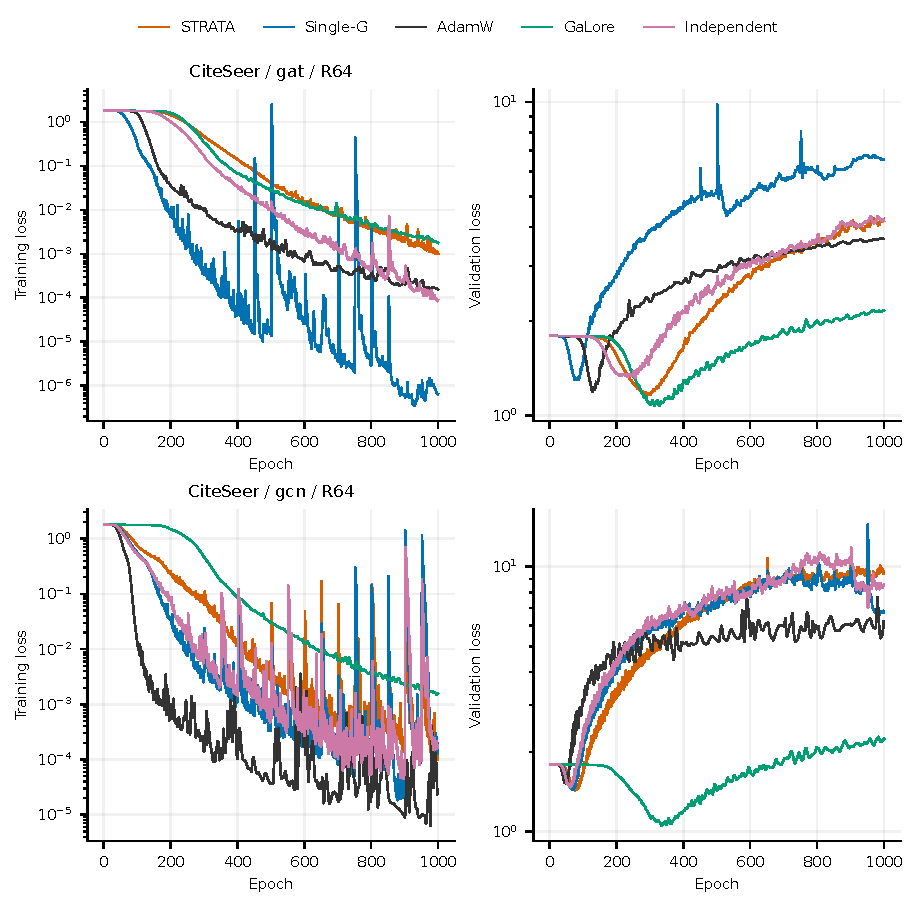
\includegraphics[width=.98\linewidth]{figures/fig_breadth_complete_00.pdf}
\caption{\textbf{Completed breadth-cohort training and validation losses.} CiteSeer/gat: two-rate validation selection; CiteSeer/gcn: two-rate validation selection. Left: training; right: validation. Raw complete trajectories, seed 42. No smoothing or extrapolation.}
\end{figure}
\begin{figure}[!htbp]
\centering
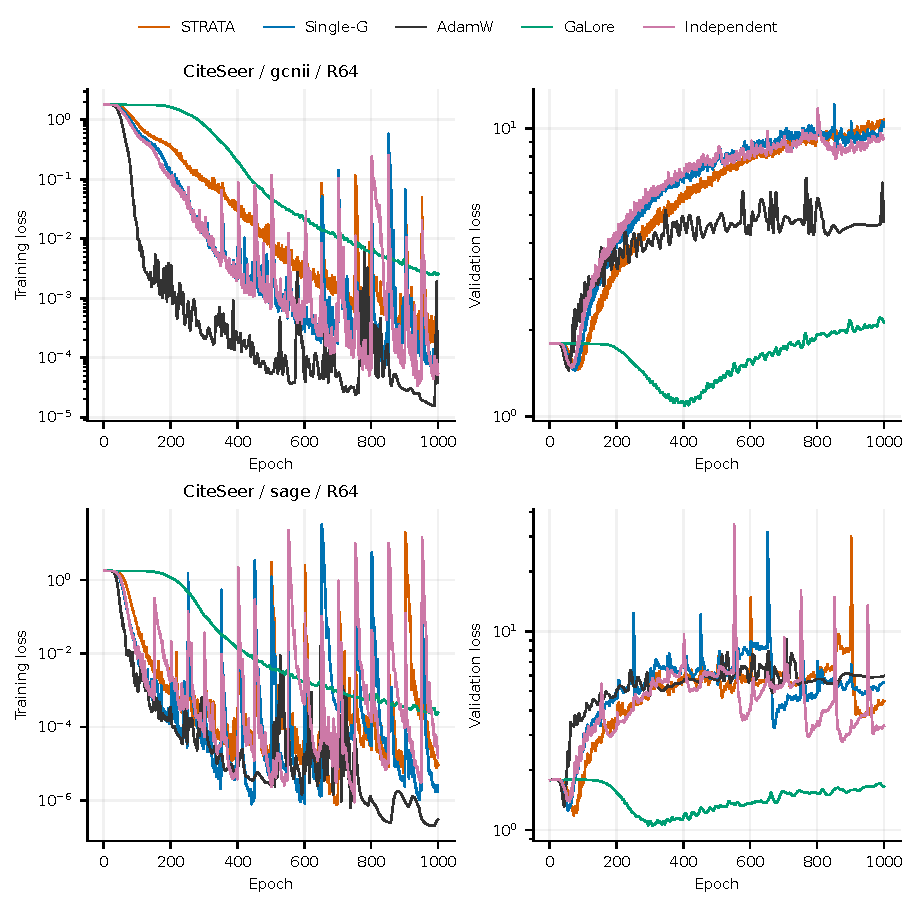
\includegraphics[width=.98\linewidth]{figures/fig_breadth_complete_01.pdf}
\caption{\textbf{Completed breadth-cohort training and validation losses.} CiteSeer/gcnii: two-rate validation selection; CiteSeer/sage: two-rate validation selection. Left: training; right: validation. Raw complete trajectories, seed 42. No smoothing or extrapolation.}
\end{figure}
\begin{figure}[!htbp]
\centering
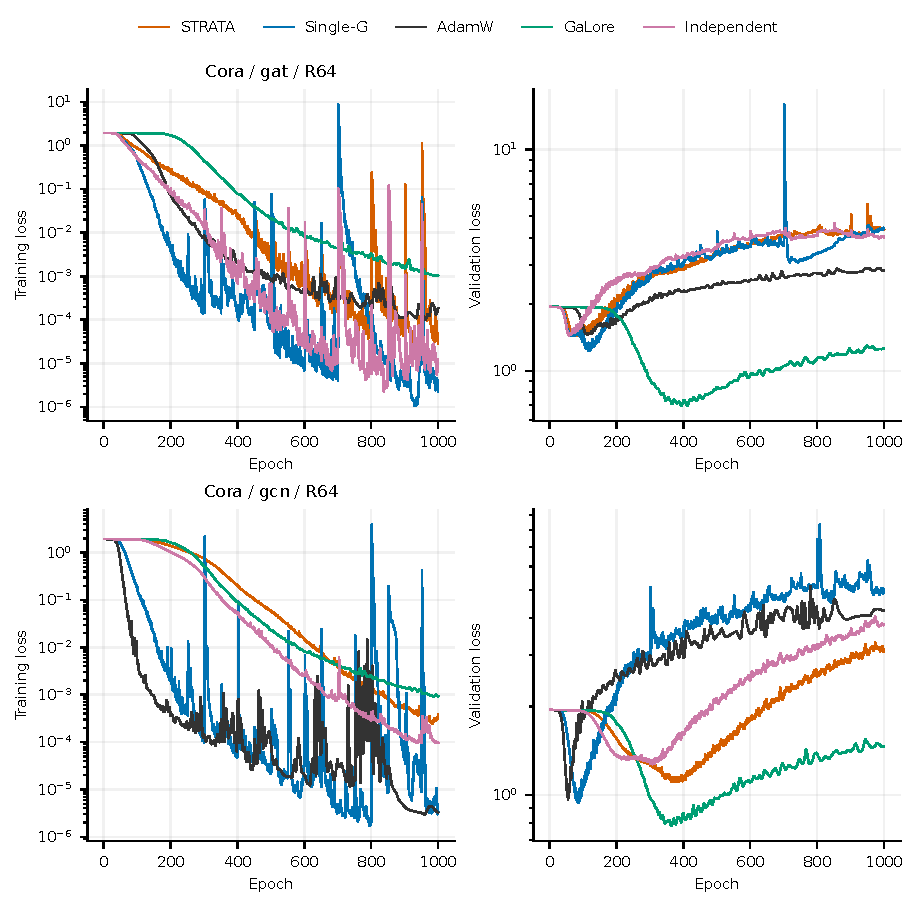
\includegraphics[width=.98\linewidth]{figures/fig_breadth_complete_02.pdf}
\caption{\textbf{Completed breadth-cohort training and validation losses.} Cora/gat: two-rate validation selection; Cora/gcn: two-rate validation selection. Left: training; right: validation. Raw complete trajectories, seed 42. No smoothing or extrapolation.}
\end{figure}
\begin{figure}[!htbp]
\centering
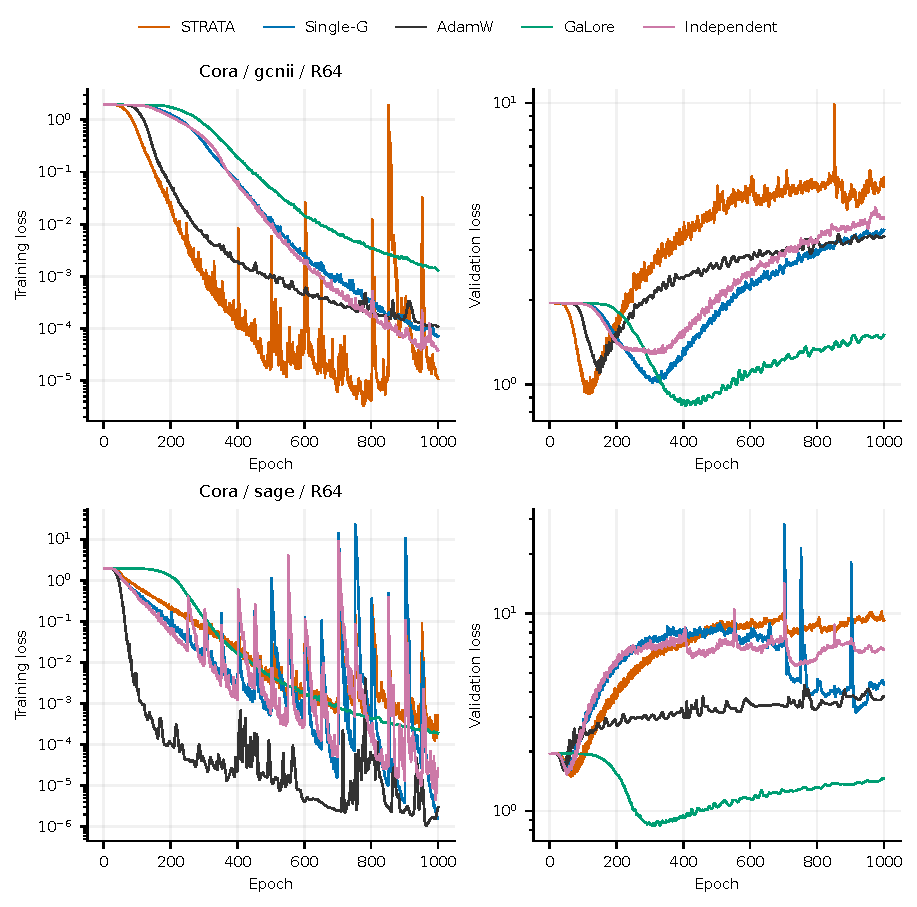
\includegraphics[width=.98\linewidth]{figures/fig_breadth_complete_03.pdf}
\caption{\textbf{Completed breadth-cohort training and validation losses.} Cora/gcnii: two-rate validation selection; Cora/sage: two-rate validation selection. Left: training; right: validation. Raw complete trajectories, seed 42. No smoothing or extrapolation.}
\end{figure}
\begin{figure}[!htbp]
\centering
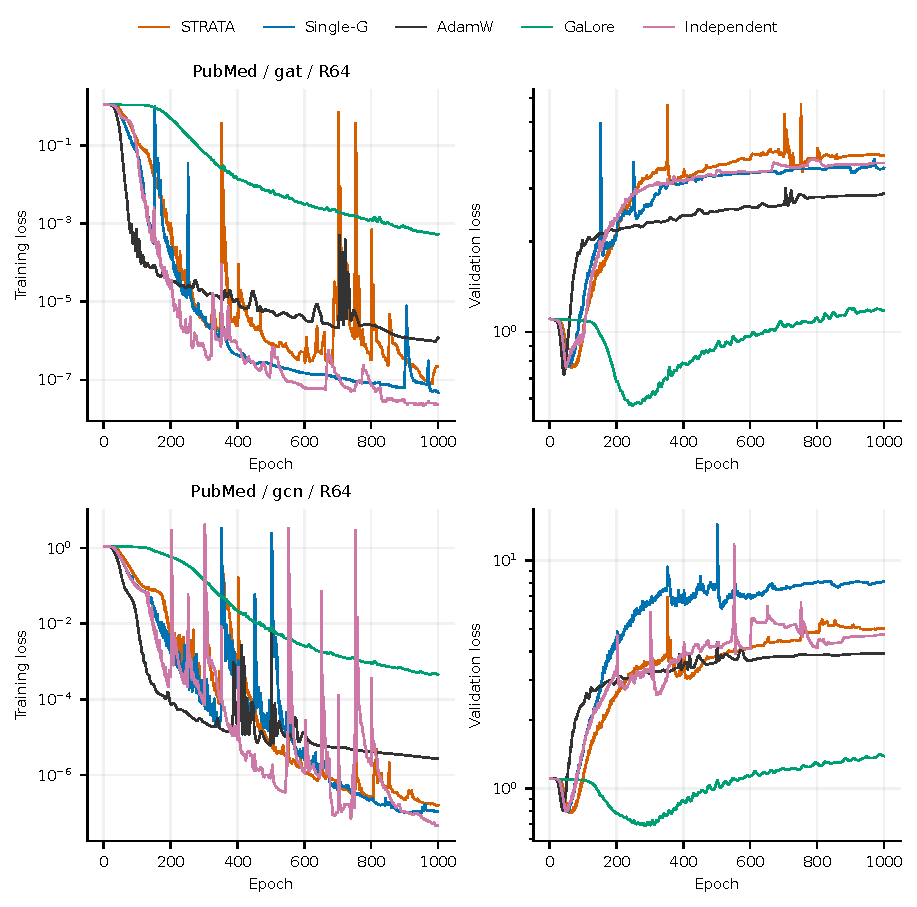
\includegraphics[width=.98\linewidth]{figures/fig_breadth_complete_04.pdf}
\caption{\textbf{Completed breadth-cohort training and validation losses.} PubMed/gat: two-rate validation selection; PubMed/gcn: two-rate validation selection. Left: training; right: validation. Raw complete trajectories, seed 42. No smoothing or extrapolation.}
\end{figure}
\begin{figure}[!htbp]
\centering
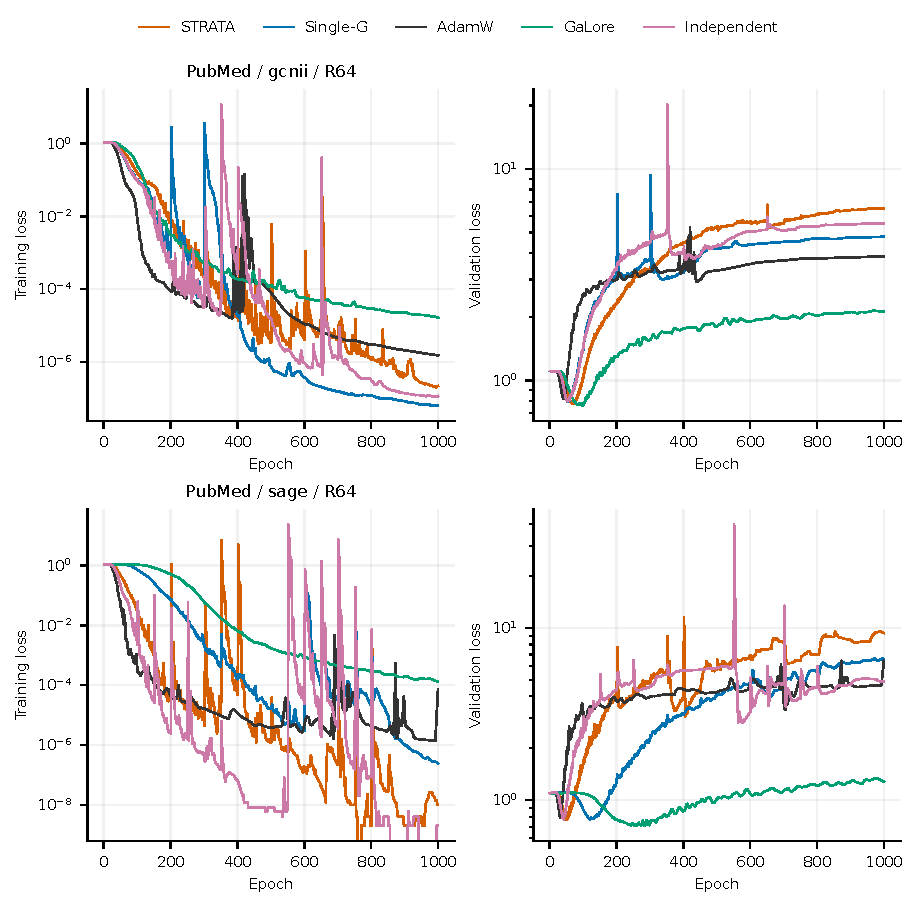
\includegraphics[width=.98\linewidth]{figures/fig_breadth_complete_05.pdf}
\caption{\textbf{Completed breadth-cohort training and validation losses.} PubMed/gcnii: two-rate validation selection; PubMed/sage: two-rate validation selection. Left: training; right: validation. Raw complete trajectories, seed 42. No smoothing or extrapolation.}
\end{figure}
\begin{figure}[!htbp]
\centering
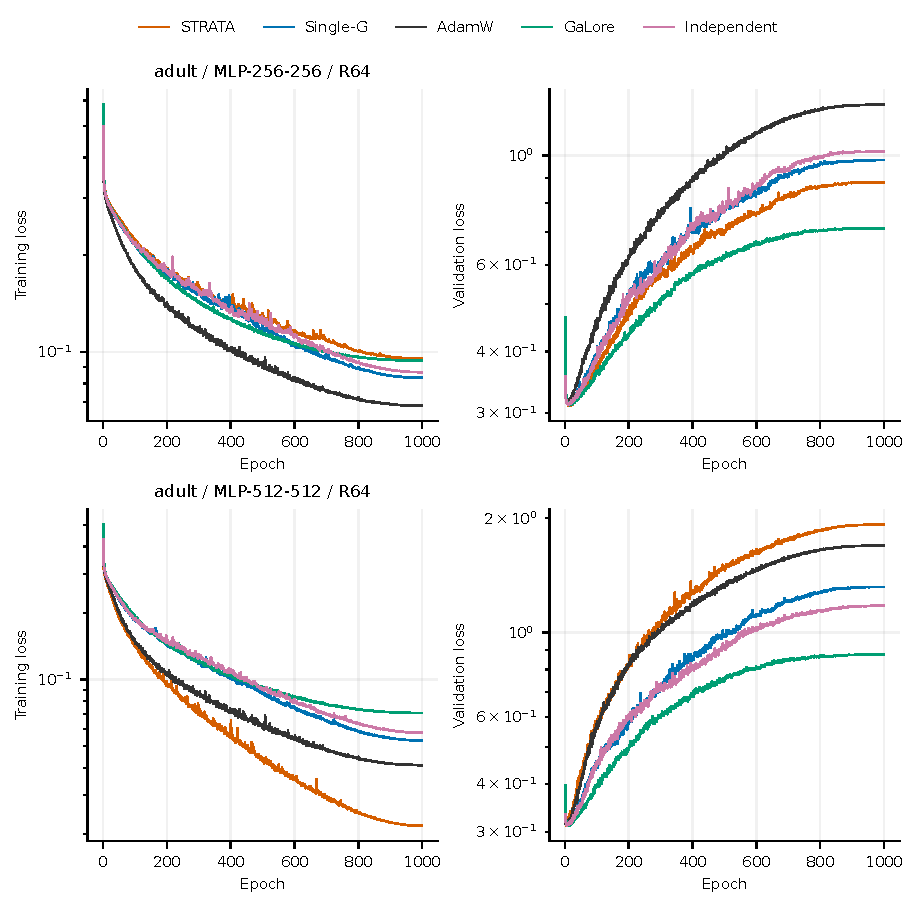
\includegraphics[width=.98\linewidth]{figures/fig_breadth_complete_06.pdf}
\caption{\textbf{Completed breadth-cohort training and validation losses.} adult/MLP-256-256: two-rate validation selection; adult/MLP-512-512: two-rate validation selection. Left: training; right: validation. Raw complete trajectories, seed 42. No smoothing or extrapolation.}
\end{figure}
\begin{figure}[!htbp]
\centering
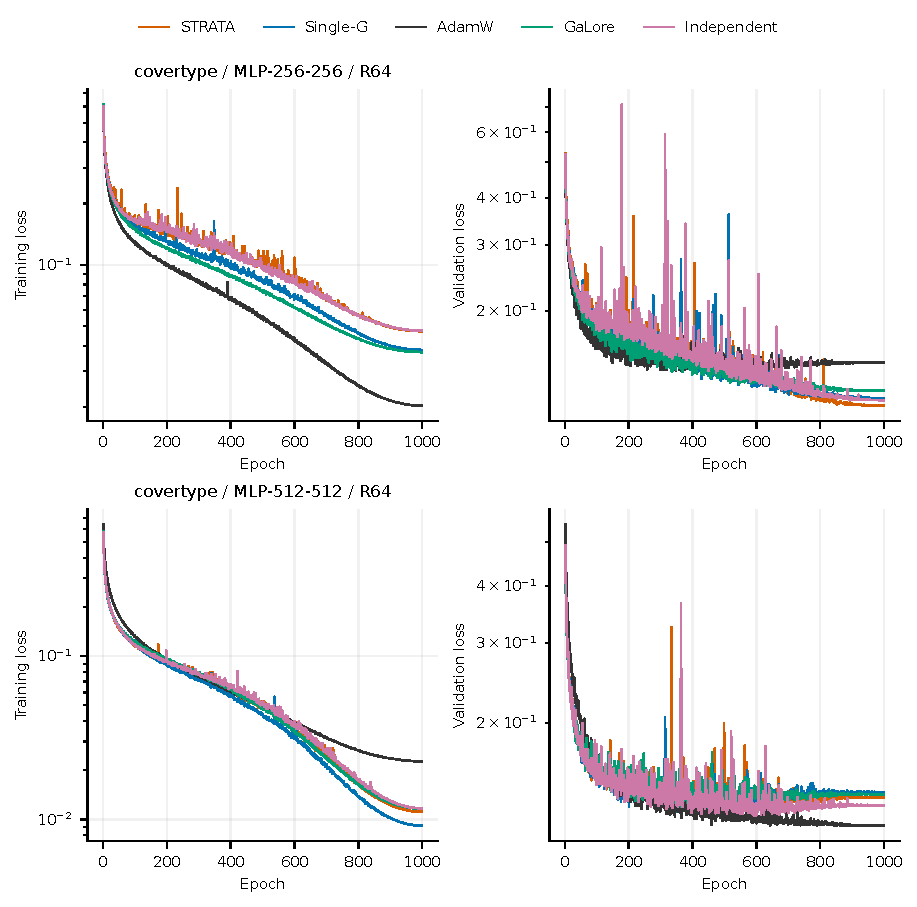
\includegraphics[width=.98\linewidth]{figures/fig_breadth_complete_07.pdf}
\caption{\textbf{Completed breadth-cohort training and validation losses.} covertype/MLP-256-256: two-rate validation selection; covertype/MLP-512-512: two-rate validation selection. Left: training; right: validation. Raw complete trajectories, seed 42. No smoothing or extrapolation.}
\end{figure}
\begin{figure}[!htbp]
\centering
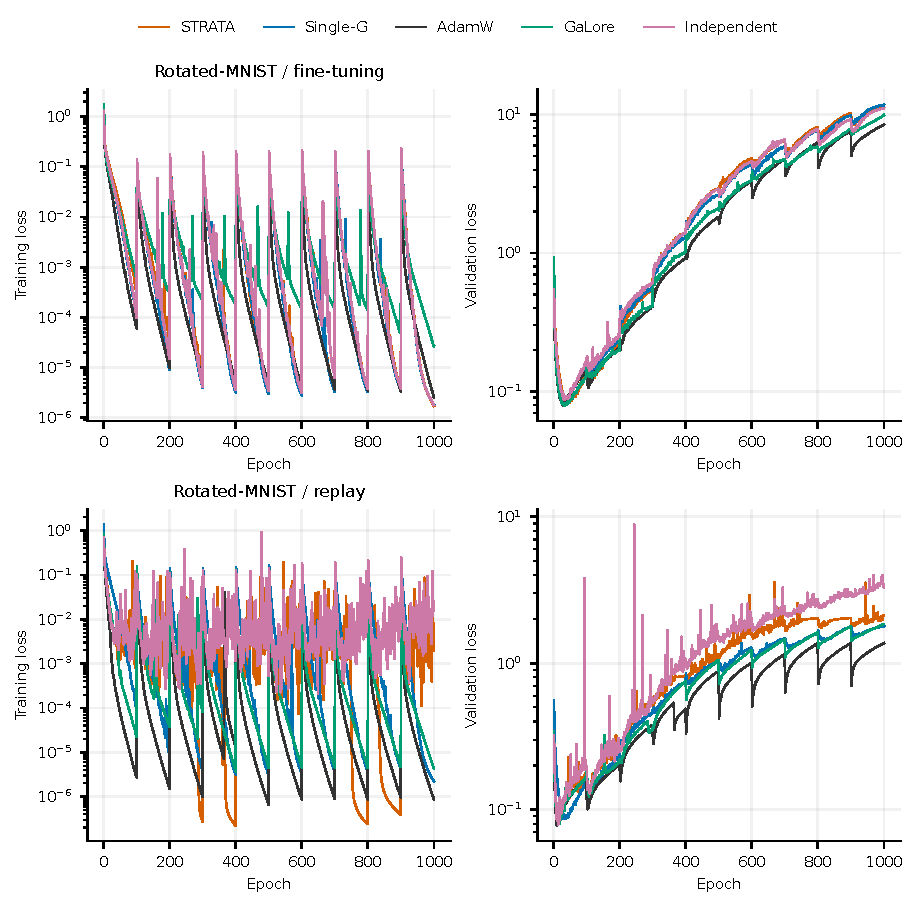
\includegraphics[width=.98\linewidth]{figures/fig_breadth_complete_08.pdf}
\caption{\textbf{Completed breadth-cohort training and validation losses.} rotated\_mnist\_cl/MLP-256-256/finetune: two-rate validation selection; rotated\_mnist\_cl/MLP-256-256/replay: two-rate validation selection. Left: training; right: validation. Raw complete trajectories, seed 42. Continual validation averages seen tasks, so its evaluation distribution changes at task boundaries. No smoothing or extrapolation.}
\end{figure}
\begin{figure}[!htbp]
\centering
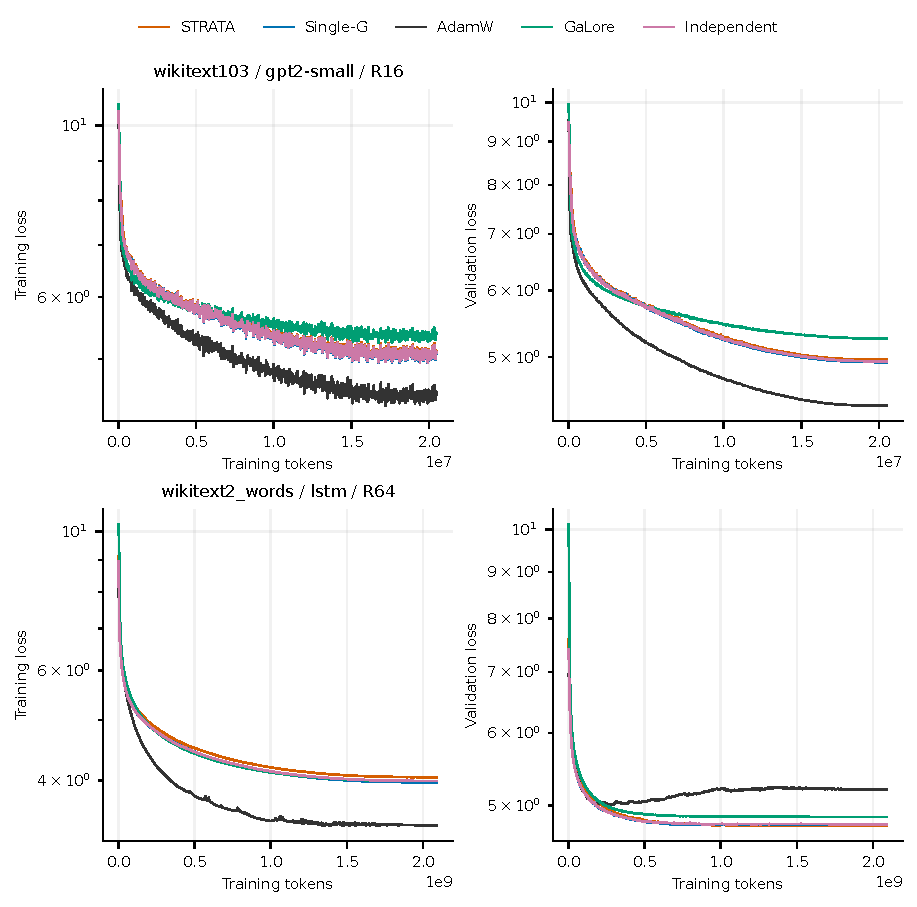
\includegraphics[width=.98\linewidth]{figures/fig_breadth_complete_09.pdf}
\caption{\textbf{Completed breadth-cohort training and validation losses.} wikitext103/gpt2-small: two-rate validation selection; wikitext2\_words/lstm: fixed rate 0.0003; search incomplete. Left: training; right: validation. Raw complete trajectories, seed 42. No smoothing or extrapolation.}
\end{figure}
\begin{figure}[!htbp]
\centering
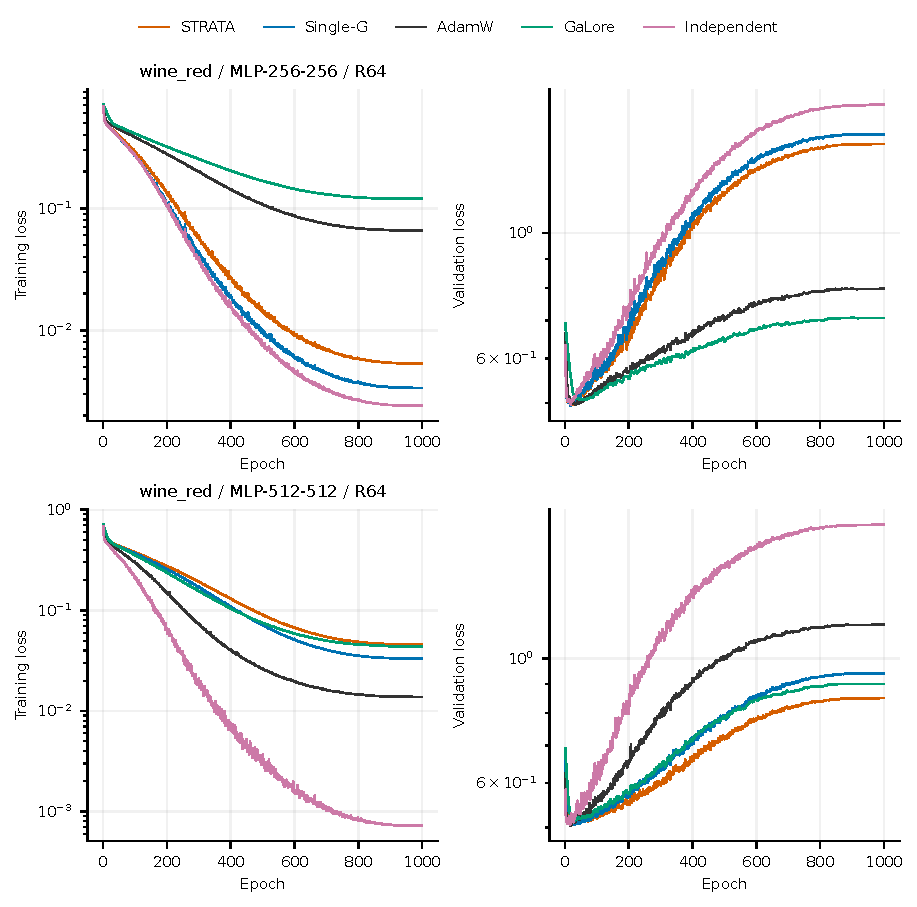
\includegraphics[width=.98\linewidth]{figures/fig_breadth_complete_10.pdf}
\caption{\textbf{Completed breadth-cohort training and validation losses.} wine\_red/MLP-256-256: two-rate validation selection; wine\_red/MLP-512-512: two-rate validation selection. Left: training; right: validation. Raw complete trajectories, seed 42. No smoothing or extrapolation.}
\end{figure}
\begin{figure}[!htbp]
\centering
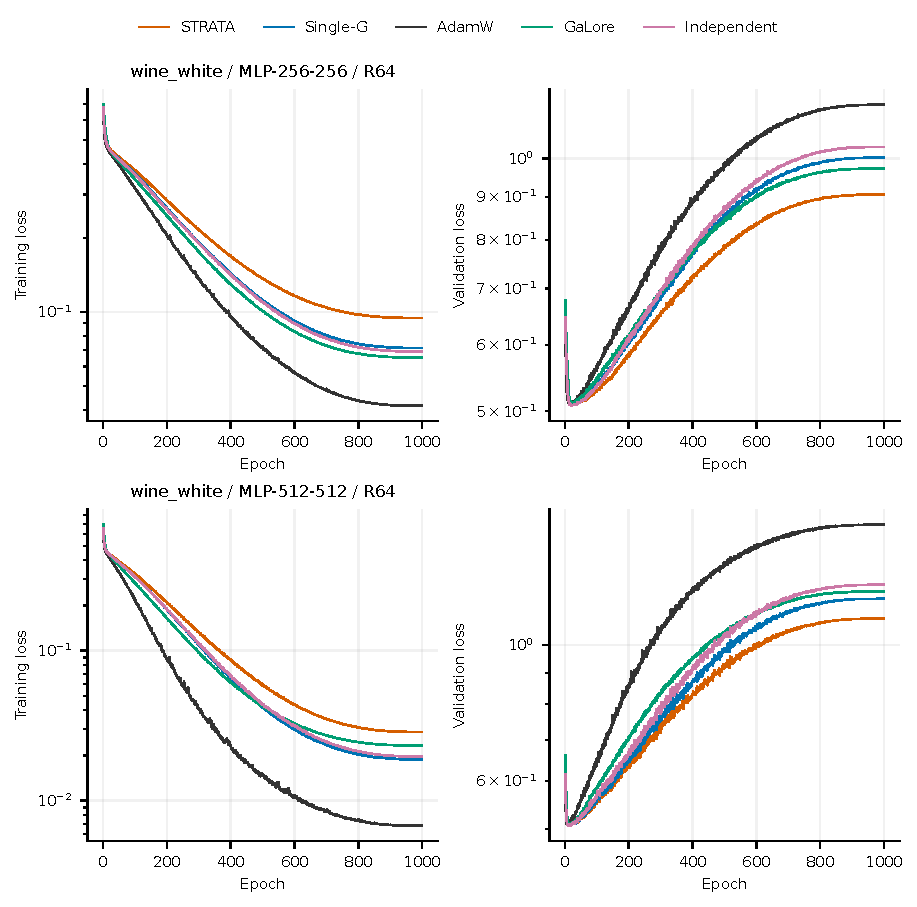
\includegraphics[width=.98\linewidth]{figures/fig_breadth_complete_11.pdf}
\caption{\textbf{Completed breadth-cohort training and validation losses.} wine\_white/MLP-256-256: two-rate validation selection; wine\_white/MLP-512-512: two-rate validation selection. Left: training; right: validation. Raw complete trajectories, seed 42. No smoothing or extrapolation.}
\end{figure}


\FloatBarrier
\subsection{Completed ablation loss trajectories}
Each panel uses one predeclared fixed learning rate and only full-budget completed runs. The ablation matrix may still be incomplete; missing variants are not assigned values. All completed variants, including adverse ones, are retained.
\begin{figure}[!htbp]
\centering
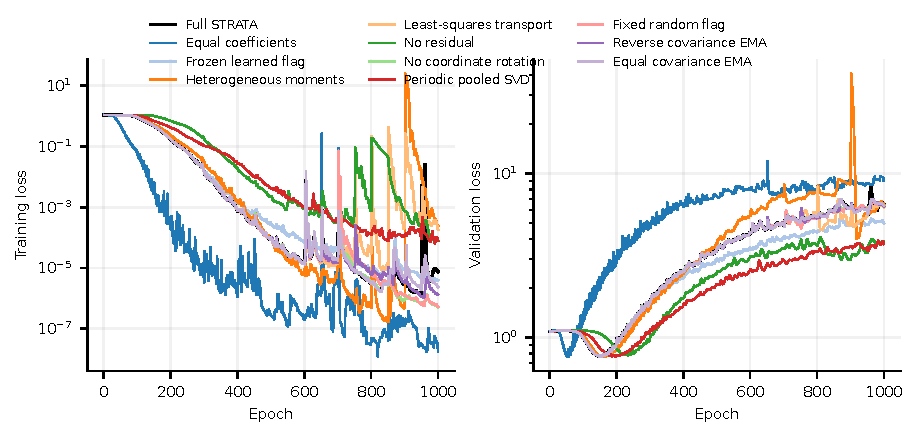
\includegraphics[width=.98\linewidth]{figures/fig_ablation_complete_f4222fea23ff.pdf}
\caption{\textbf{Completed fixed-rate ablation trajectories.} PubMed/sage/64/0.0003. Left: training; right: validation. Raw losses for the full method and every currently completed variant, seed 42. No smoothing, test selection or extrapolation. In continual learning the validation set averages seen tasks.}
\end{figure}
\begin{figure}[!htbp]
\centering
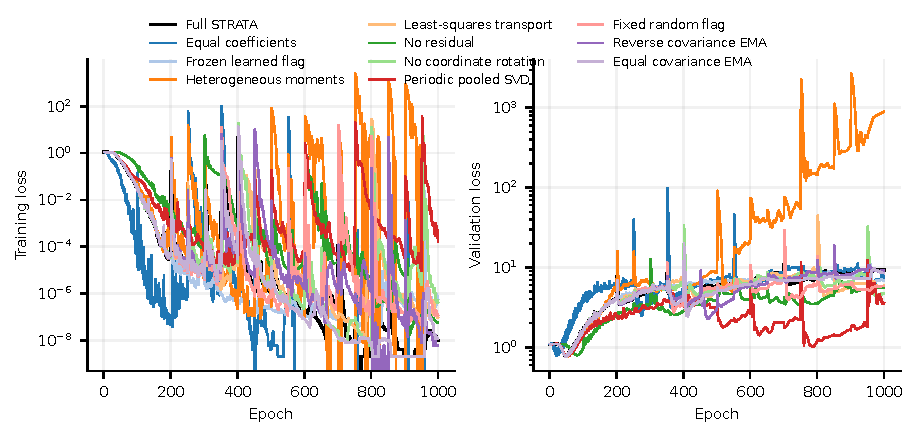
\includegraphics[width=.98\linewidth]{figures/fig_ablation_complete_92ad161e923b.pdf}
\caption{\textbf{Completed fixed-rate ablation trajectories.} PubMed/sage/64/0.001. Left: training; right: validation. Raw losses for the full method and every currently completed variant, seed 42. No smoothing, test selection or extrapolation. In continual learning the validation set averages seen tasks.}
\end{figure}
\begin{figure}[!htbp]
\centering
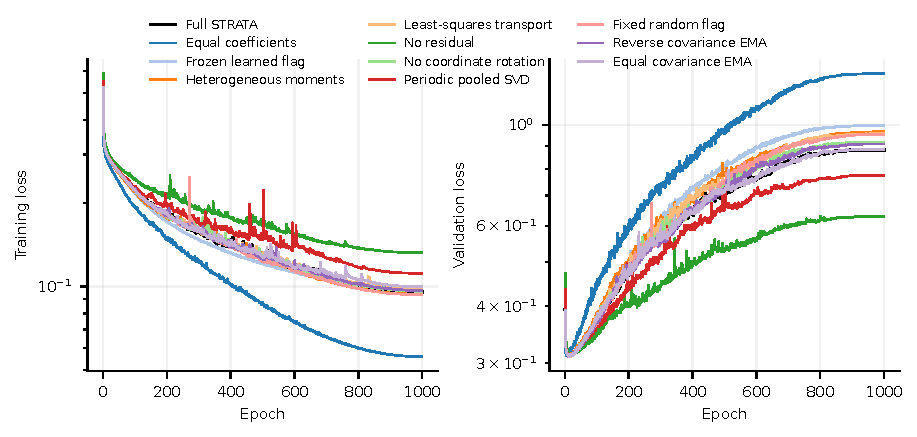
\includegraphics[width=.98\linewidth]{figures/fig_ablation_complete_cd63c9d43c42.pdf}
\caption{\textbf{Completed fixed-rate ablation trajectories.} adult/MLP-256-256/64/0.0003. Left: training; right: validation. Raw losses for the full method and every currently completed variant, seed 42. No smoothing, test selection or extrapolation. In continual learning the validation set averages seen tasks.}
\end{figure}
\begin{figure}[!htbp]
\centering
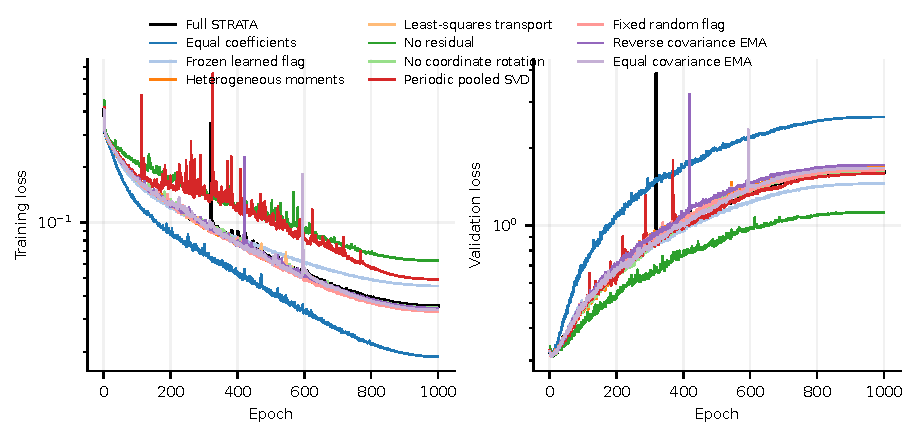
\includegraphics[width=.98\linewidth]{figures/fig_ablation_complete_f1b02595ebb0.pdf}
\caption{\textbf{Completed fixed-rate ablation trajectories.} adult/MLP-256-256/64/0.001. Left: training; right: validation. Raw losses for the full method and every currently completed variant, seed 42. No smoothing, test selection or extrapolation. In continual learning the validation set averages seen tasks.}
\end{figure}
\begin{figure}[!htbp]
\centering
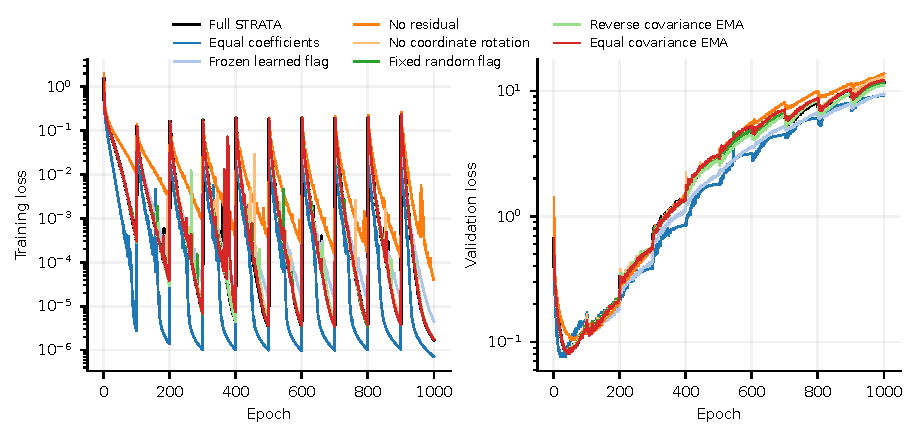
\includegraphics[width=.98\linewidth]{figures/fig_ablation_complete_22095cc4347a.pdf}
\caption{\textbf{Completed fixed-rate ablation trajectories.} rotated\_mnist\_cl/MLP-256-256/64/0.0003. Left: training; right: validation. Raw losses for the full method and every currently completed variant, seed 42. No smoothing, test selection or extrapolation. In continual learning the validation set averages seen tasks.}
\end{figure}
\begin{figure}[!htbp]
\centering
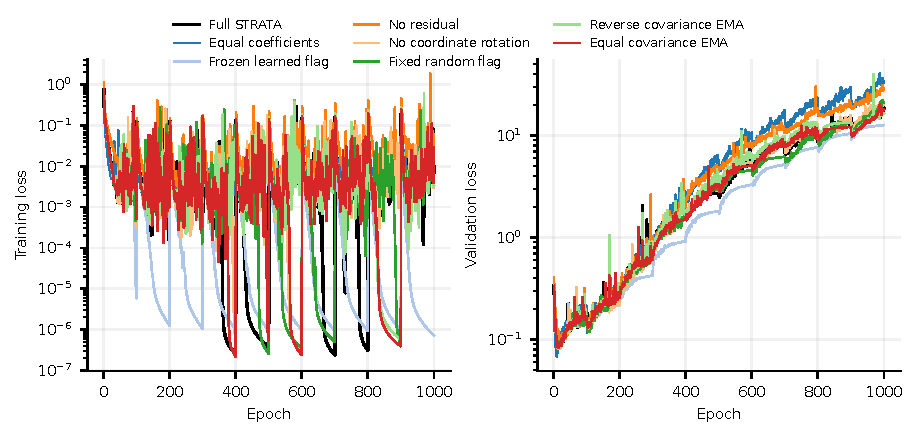
\includegraphics[width=.98\linewidth]{figures/fig_ablation_complete_4cf87464d8ba.pdf}
\caption{\textbf{Completed fixed-rate ablation trajectories.} rotated\_mnist\_cl/MLP-256-256/64/0.001. Left: training; right: validation. Raw losses for the full method and every currently completed variant, seed 42. No smoothing, test selection or extrapolation. In continual learning the validation set averages seen tasks.}
\end{figure}
\begin{figure}[!htbp]
\centering
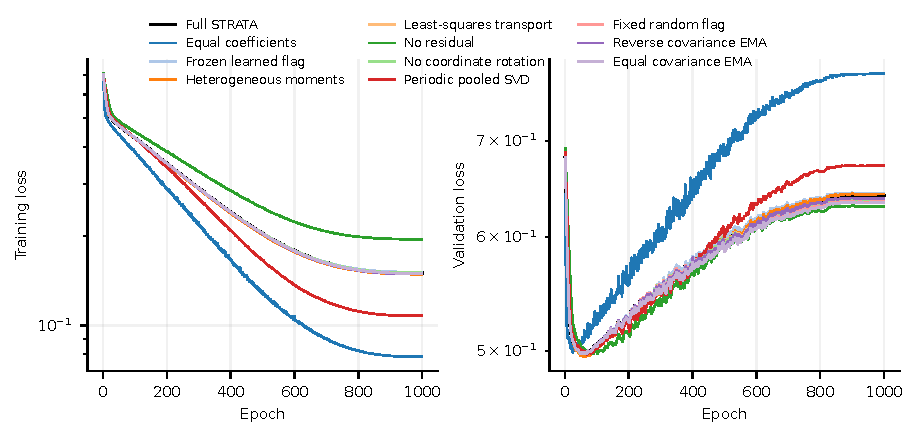
\includegraphics[width=.98\linewidth]{figures/fig_ablation_complete_6327e4845709.pdf}
\caption{\textbf{Completed fixed-rate ablation trajectories.} wine\_red/MLP-256-256/64/0.0003. Left: training; right: validation. Raw losses for the full method and every currently completed variant, seed 42. No smoothing, test selection or extrapolation. In continual learning the validation set averages seen tasks.}
\end{figure}
\begin{figure}[!htbp]
\centering
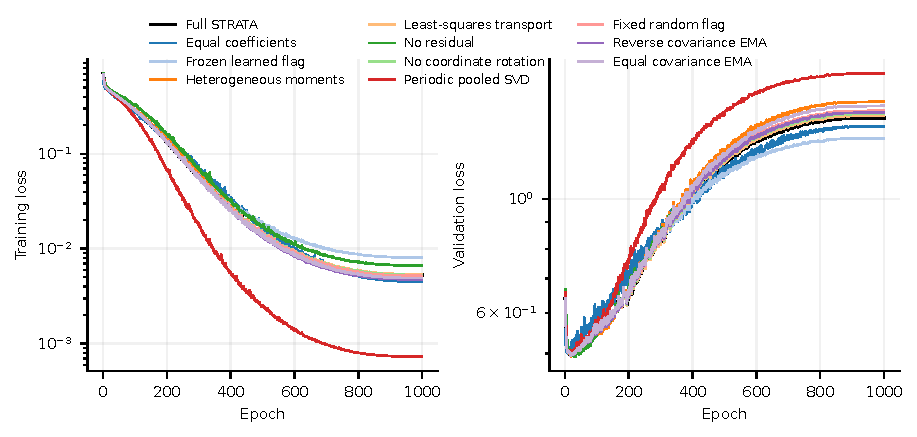
\includegraphics[width=.98\linewidth]{figures/fig_ablation_complete_f7dd6296b414.pdf}
\caption{\textbf{Completed fixed-rate ablation trajectories.} wine\_red/MLP-256-256/64/0.001. Left: training; right: validation. Raw losses for the full method and every currently completed variant, seed 42. No smoothing, test selection or extrapolation. In continual learning the validation set averages seen tasks.}
\end{figure}

